\chapter{Sintesis: Rendemen dan Kemurnian}\label{ch:g10:synthesis-yield}

Aspirin adalah salah satu obat yang paling banyak dipakai di dunia.
Kisahnya bermula dari kulit pohon dedalu, yang sejak lama dikunyah untuk
melawan nyeri dan demam; zat aktif dalam kulit pohon itu dilacak, pada
abad kesembilan belas, sampai ke sekelompok senyawa yang darinya para
ahli kimia membuat asam salisilat. Karena terlalu keras bagi lambung
untuk diminum dalam dosis besar, asam salisilat diubah menjadi zat yang
lebih lembut, asam asetilsalisilat: aspirin. Kini aspirin dibuat
berton-ton di dalam reaktor baja, dengan reaksi yang sama yang dapat
dilakukan laboratorium sekolah dalam satu sore. Membuat sebuah zat baru
separuh pekerjaan: zat itu juga harus dipisahkan dari segala sesuatu
yang lain di dalam labu, dimurnikan, diperiksa, dan ditimbang untuk
melihat berapa banyak dari yang mungkin benar-benar telah diperoleh.

\begin{recall}
\omterm{def:g10:chemical-species:extraction}{Ekstraksi}, \omterm{def:g10:chemical-species:distillation}{distilasi}, \omterm{def:g10:chemical-species:tlc}{kromatografi lapis tipis} dan \omterm{def:g10:chemical-species:retention-factor}{faktor retensi};
padatan murni meleleh pada suhu yang tajam dan diketahui
(\cref{ch:g10:chemical-species}). Saringan menahan padatan dan
meloloskan cairan (\cref{ch:g3:separating-mixtures}). \omterm{def:g10:reaction-progress-table:extent}{Tabel kemajuan}
memberikan jumlah produk terbesar dari \omterm{def:g10:reaction-progress-table:limiting}{pereaksi pembatas}
(\cref{ch:g10:reaction-progress-table}).
\end{recall}

\begin{omfigure}
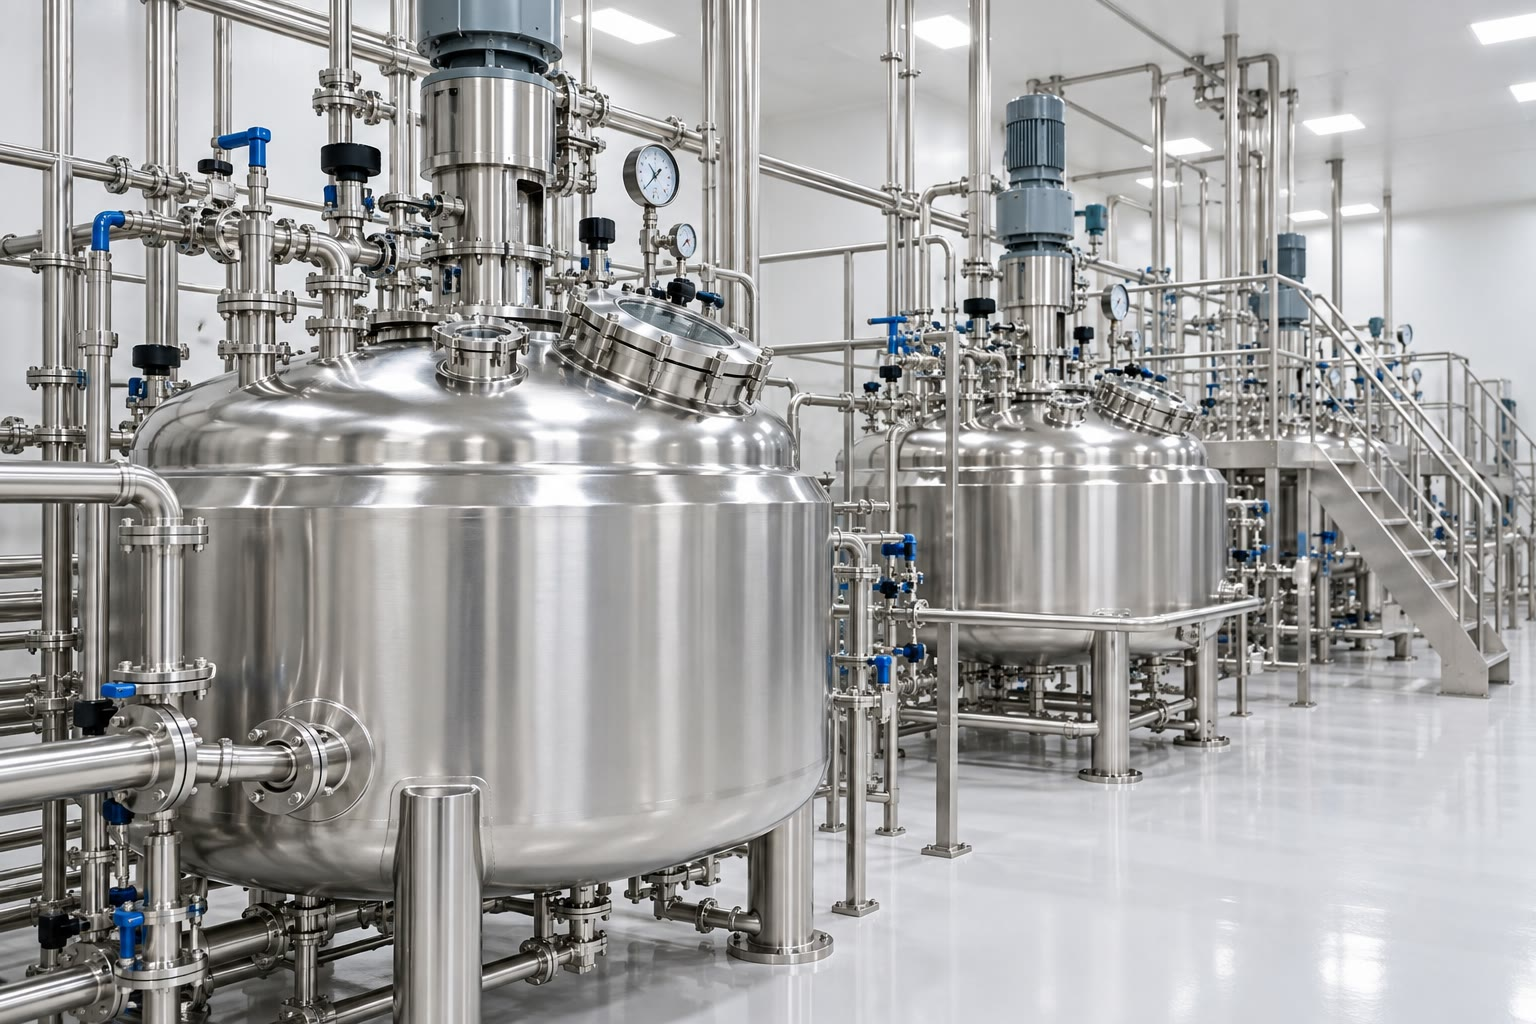
\includegraphics[width=0.55\linewidth]{images/book1/ai/g10-pharma-reactor.jpg}

{\small Reaktor baja di pabrik farmasi: \omterm{def:g10:synthesis-yield:synthesis}{sintesis} laboratorium, yang
diperbesar sejuta kali.}
\end{omfigure}

\section{Langkah-langkah sintesis}

\begin{definition}[Sintesis, produk kasar]\label{def:g10:synthesis-yield:synthesis}
Yang disebut \emph{sintesis}\index{sintesis} adalah pembuatan sebuah
\omterm{def:g6:pure-substances-and-mixtures:species}{spesies kimia} melalui satu atau beberapa \omterm{def:g7:chemical-reactions:reaction}{reaksi kimia}, mulai dari
spesies-spesies lain. Padatan atau cairan yang diperoleh langsung dari
\omterm{def:g6:pure-substances-and-mixtures:mixture}{campuran} reaksi, sebelum dimurnikan sama sekali, disebut
\emph{produk kasar}\index{produk kasar}: produk itu masih mengandung
\omterm{def:g7:chemical-reactions:reactant}{pereaksi}, produk samping, dan \omterm{def:g6:solutions-and-solubility:solute}{pelarut}.
\end{definition}

\begin{method}[Merencanakan sintesis]\label{met:g10:synthesis-yield:plan}
Sebuah \omterm{def:g10:synthesis-yield:synthesis}{sintesis} dilakukan dalam empat langkah:
\begin{enumerate}
  \item \textbf{Reaksi}: \omterm{def:g2:mixing-and-dissolving:mix}{campurkan} \omterm{def:g7:chemical-reactions:reactant}{pereaksi} dalam jumlah yang tepat,
        sering dengan salah satunya berlebih, dan panaskan jika perlu.
  \item \textbf{Isolasi}: pisahkan \omterm{def:g10:synthesis-yield:synthesis}{produk kasar} dari \omterm{def:g6:pure-substances-and-mixtures:mixture}{campuran} reaksi
        (\omterm{def:g3:separating-mixtures:filter}{penyaringan}, \omterm{def:g10:chemical-species:extraction}{ekstraksi}).
  \item \textbf{Pemurnian}: hilangkan pengotor dari \omterm{def:g10:synthesis-yield:synthesis}{produk kasar}
        (\omterm{def:g10:synthesis-yield:recrystallisation}{rekristalisasi} untuk padatan, \omterm{def:g10:chemical-species:distillation}{distilasi} untuk cairan).
  \item \textbf{Analisis}: periksalah identitas dan kemurnian produk
        (titik leleh, kromatografi), lalu timbang dan hitung
        \omterm{def:g10:synthesis-yield:yield}{rendemennya}.
\end{enumerate}
\end{method}

\begin{example}[Membuat aspirin]\label{ex:g10:synthesis-yield:aspirin}
Asam salisilat bereaksi dengan anhidrida etanoat (juga disebut
anhidrida asetat) menghasilkan aspirin dan asam etanoat:
\[
  \ce{C7H6O3 + C4H6O3 -> C9H8O4 + C2H4O2}
\]
\[
  \text{asam salisilat} + \text{anhidrida etanoat} \longrightarrow
  \text{aspirin} + \text{asam etanoat}.
\]
Anhidridanya dibuat berlebih, agar semua asam salisilat bereaksi; asam
etanoat yang terbentuk adalah produk samping.
\end{example}

\begin{omfigure}
\setchemfig{atom sep=1.7em}
\begin{tabular}{@{}c@{\enspace}c@{\enspace}c@{\enspace}c@{\enspace}c@{\enspace}c@{\enspace}c@{}}
\chemfig{*6(-=-(-COOH)=(-OH)-=)} & $+$ &
\chemfig{H_3C-C(=[2]O)-O-C(=[2]O)-CH_3} & $\longrightarrow$ &
\chemfig{*6(-=-(-COOH)=(-O-[:150]C(=[:90]O)-[:210]H_3C)-=)} & $+$ &
\chemfig{H_3C-C(=[2]O)-OH} \\[2pt]
\small asam salisilat & & \small anhidrida etanoat & &
\small aspirin & & \small asam etanoat
\end{tabular}\par\medskip

{\small Pembuatan aspirin, dengan rumus yang digambar (setiap sudut
segi enam adalah \omterm{def:g7:atoms-and-molecules:atom}{atom} karbon, yang mengikat sebuah \omterm{def:g7:atoms-and-molecules:atom}{atom} hidrogen di
tempat yang tidak digambar apa pun; sebuah bab berikutnya menjelaskan
cara penulisan singkat ini). Gugus \ce{-OH} pada cincin asam salisilat
mengambil separuh anhidrida; separuh yang lain pergi sebagai asam
etanoat.}
\end{omfigure}

\section{Pemanasan dengan refluks}

\begin{definition}[Pemanasan dengan refluks]\label{def:g10:synthesis-yield:reflux}
Yang disebut \emph{pemanasan dengan refluks}\index{pemanasan dengan refluks}
adalah memanaskan \omterm{def:g6:pure-substances-and-mixtures:mixture}{campuran} reaksi dalam sebuah labu yang di atasnya
dipasang kondensor tegak: uapnya naik, mendingin di dalam kondensor,
dan cairannya mengalir kembali ke dalam labu.
\end{definition}

\begin{proposition}[Mengapa refluks]\label{prop:g10:synthesis-yield:why-reflux}
Pemanasan mempercepat kebanyakan reaksi; refluks memungkinkan pemanasan
selama yang diperlukan pada suhu didih \omterm{def:g6:pure-substances-and-mixtures:mixture}{campuran} tanpa kehilangan
\omterm{def:g7:chemical-reactions:reactant}{pereaksi}, produk, atau \omterm{def:g6:solutions-and-solubility:solute}{pelarut} sebagai uap.
\end{proposition}

\begin{proof}
Suhu cairan yang mendidih tidak dapat naik melebihi titik didihnya, dan
setiap uap yang lolos dari cairan diembunkan dan dikembalikan: tidak
ada yang meninggalkan peralatan itu, yang tetap terbuka di bagian atas
agar tidak ada tekanan yang menumpuk.
\end{proof}

\begin{omfigure}
\begin{tikzpicture}[font=\small, scale=1.05]
  \pic[transform shape] at (0,0) {heatingmantle};
  \pic[transform shape] at (0,0) {rbflask={0.42}{orange!25}};
  \foreach \p in {(-0.3,0.25), (0.2,0.18), (0.45,0.4), (-0.5,0.5)}
    \fill[black!45] \p circle (0.05);
  \pic[transform shape] at (0,3.0) {condenser};
  \draw[omDef, thick, <-] (0.8,3.825) -- (1.9,3.825) node[right] {air masuk};
  \draw[omDef, thick, ->] (0.8,5.375) -- (1.9,5.375) node[right] {air keluar};
  \draw[omProp, thick, <-] (-0.18,5.8) -- (-1.4,6.1) node[left] {ujung atas terbuka};
  \draw[omProp, thick, <-] (-0.45,1.2) -- (-2.0,1.6)
    node[left, align=right] {campuran reaksi\\ dan batu didih};
  \draw[omProp, thick, <-] (-1.35,-0.2) -- (-2.0,-0.6)
    node[left] {mantel pemanas};
  \draw[omThm, ->, thick] (-0.05,3.4) -- (-0.05,4.3);
  \draw[omDef, ->, thick] (0.05,4.3) -- (0.05,3.4);
  \node[omThm, anchor=east, font=\footnotesize] at (-0.45,4.6) {uap naik};
  \node[omDef, anchor=west, font=\footnotesize] at (0.85,4.6) {cairan turun kembali};
\end{tikzpicture}

{\small \omterm{def:g10:synthesis-yield:reflux}{Pemanasan dengan refluks}. Air dingin masuk ke selubung kondensor
dari bawah dan keluar dari atas, sehingga selubungnya selalu penuh.}
\end{omfigure}

\begin{remark}[Air masuk dari bawah]\label{rem:g10:synthesis-yield:water}
Jika dialirkan dari atas, air akan langsung mengalir ke bawah dan
membiarkan bagian atas selubung terisi \omterm{def:g4:air-a-mixture-of-gases:air}{udara}; jika dialirkan dari
bawah, air harus memenuhi seluruh selubung sebelum dapat keluar.
\end{remark}

\section{Mengisolasi dan memurnikan}

\begin{definition}[Penyaringan vakum]\label{def:g10:synthesis-yield:vacuum-filtration}
Yang disebut \emph{penyaringan vakum}\index{penyaringan vakum} adalah
\omterm{def:g3:separating-mixtures:filter}{penyaringan} yang cairannya ditarik menembus kertas saring dengan
pengisapan: sebuah corong datar dengan pelat berlubang-lubang (corong
Büchner) dipasang di atas labu isap yang dihubungkan ke pompa vakum.
\end{definition}

\begin{omfigure}
\begin{tikzpicture}[font=\small, scale=1.05]
  \pic[transform shape] (ff) at (0,0) {filterflask={0.12}{orange!20}};
  \fill[black!50] (-0.3,2.45) rectangle (0.3,2.8);
  \pic[transform shape] at (0,2.45) {buchner={black!8}};
  \draw[black!60, line width=2pt] (ff-arm) -- (2.6,2.2);
  \draw[omProp, thick, ->] (2.7,2.2) -- (3.4,2.2) node[right,
    align=left, text=black] {ke pompa\\ vakum};
  \draw[omProp, thick, <-] (0.7,3.8) -- (1.9,4.3) node[right, text=black]
    {kristal di atas kertas saring};
  \draw[omProp, thick, <-] (-0.4,0.15) -- (-1.8,0.6) node[left, text=black]
    {filtrat};
  \draw[omProp, thick, <-] (-0.3,2.6) -- (-1.8,2.9) node[left, text=black]
    {cincin karet};
\end{tikzpicture}

{\small \omterm{def:g10:synthesis-yield:vacuum-filtration}{Penyaringan vakum} dengan corong Büchner: pompa menarik cairan
dengan cepat dan meninggalkan padatan yang hampir kering.}
\end{omfigure}

\begin{definition}[Rekristalisasi]\label{def:g10:synthesis-yield:recrystallisation}
Yang disebut \emph{rekristalisasi}\index{rekristalisasi} adalah cara
memurnikan padatan dengan melarutkannya dalam volume \omterm{def:g6:solutions-and-solubility:solute}{pelarut} panas
sekecil mungkin, lalu membiarkan larutannya mendingin: produknya, yang
jauh lebih sukar \omterm{def:g2:mixing-and-dissolving:dissolve}{larut} dalam keadaan dingin, mengkristal, sedangkan
pengotornya, yang hanya sedikit, tetap terlarut.
\end{definition}

\begin{method}[Merekristalisasi padatan]\label{met:g10:synthesis-yield:recrystallise}
\begin{enumerate}
  \item Pilihlah \omterm{def:g6:solutions-and-solubility:solute}{pelarut} yang melarutkan produk dengan sangat baik dalam
        keadaan panas dan hampir tidak melarutkannya dalam keadaan dingin.
  \item Tambahkan \omterm{def:g6:solutions-and-solubility:solute}{pelarut} panas sedikit demi sedikit ke padatan kasar,
        tepat sampai padatan itu \omterm{def:g2:mixing-and-dissolving:dissolve}{larut} seluruhnya.
  \item Biarkan larutannya mendingin perlahan, lalu di dalam penangas
        es: kristal-kristal terbentuk.
  \item Kumpulkan kristal itu dengan \omterm{def:g10:synthesis-yield:vacuum-filtration}{penyaringan vakum}, cuci dengan
        sedikit \omterm{def:g6:solutions-and-solubility:solute}{pelarut} yang sangat dingin, lalu keringkan.
\end{enumerate}
\end{method}


\begin{omfigure}
\begin{tikzpicture}[font=\small]
  % 1. crude solid + a little hot solvent, on a hot plate
  \pic at (0,0.3) {hotplate};
  \pic at (0,0.3) {erlenmeyer={0.18}{orange!12}};
  \foreach \p in {(-0.4,0.42),(-0.15,0.38),(0.1,0.45),(0.35,0.4),(-0.3,0.55),(0.2,0.6)}
    \fill[brown!60] \p circle (0.06);
  \node[align=center, anchor=north] at (0,-0.15) {1. padatan\\ kasar, pelarut\\ panas};
  % 2. clear hot solution
  \pic at (3,0.3) {hotplate};
  \pic at (3,0.3) {erlenmeyer={0.22}{orange!12}};
  \node[align=center, anchor=north] at (3,-0.15) {2. larut semua,\\ jernih, panas};
  % 3. ice bath: crystals
  \fill[cyan!12, draw=black!40] (5.0,0) rectangle (7.0,1.2);
  \foreach \p in {(5.2,0.9),(6.75,1.0),(5.3,0.3),(6.8,0.25)}
    \draw[black!35, fill=white] \p ++(-0.12,-0.1) rectangle ++(0.24,0.2);
  \pic at (6,0.1) {erlenmeyer={0.2}{orange!8}};
  \foreach \x/\y in {-0.45/0.18,-0.25/0.15,0/0.2,0.25/0.15,0.45/0.2,-0.1/0.3,0.15/0.32,
                     -0.35/0.32,0.35/0.33}
    \fill[white, draw=black!55] (6+\x,0.1+\y) -- ++(0.07,0.06) -- ++(0.07,-0.06)
      -- ++(-0.07,-0.06) -- cycle;
  \node[align=center, anchor=north] at (6,-0.15) {3. dinginkan\\ dalam es:\\ mengkristal};
  % 4. filter
  \pic at (9,0) {filterflask={0.12}{orange!12}};
  \pic at (9,2.45) {buchner={black!12}};
  \fill[black!50] (8.7,2.45) rectangle (9.3,2.8);
  \node[align=center, anchor=north] at (9,-0.15) {4. saring vakum,\\ cuci dingin,\\ keringkan};
\end{tikzpicture}

{\small \omterm{def:g10:synthesis-yield:recrystallisation}{Rekristalisasi} dalam empat langkah. Pengotor tetap terlarut dalam
\omterm{def:g6:solutions-and-solubility:solute}{pelarut} dingin dan ikut ke dalam \omterm{def:g3:separating-mixtures:filter}{filtrat}.}
\end{omfigure}

\begin{remark}[Kehilangan tidak dapat dihindari]\label{rem:g10:synthesis-yield:losses}
% ledger: sol:aspirin-25, sol:aspirin-37
Bahkan dalam keadaan dingin, \omterm{def:g6:solutions-and-solubility:solute}{pelarut} tetap melarutkan sebagian produk.
Aspirin \omterm{def:g2:mixing-and-dissolving:dissolve}{larut} dalam air sekitar \qty{3.3}{g/L} pada \qty{25}{\celsius},
tiga kali lebih banyak pada \qty{37}{\celsius}, dan jauh lebih banyak
jika lebih panas: setiap mililiter \omterm{def:g3:separating-mixtures:filter}{filtrat} dan air cucian membawa pergi
sedikit aspirin. \omterm{def:g10:synthesis-yield:recrystallisation}{Rekristalisasi} membeli kemurnian dengan harga massa.
\end{remark}

\section{Menganalisis produk}

\begin{proposition}[Dua pemeriksaan kemurnian]\label{prop:g10:synthesis-yield:checks}
Padatan hasil \omterm{def:g10:synthesis-yield:synthesis}{sintesis} murni, dalam batas uji-uji ini, jika:
\begin{itemize}
  \item padatan itu meleleh dengan tajam pada titik leleh yang tercantum
        dalam tabel;
  \item pada pelat \omterm{def:g10:chemical-species:tlc}{kromatografi lapis tipis}, padatan itu memberikan satu
        bercak saja, setinggi sampel \omterm{def:g6:pure-substances-and-mixtures:pure-substance}{zat murninya}.
\end{itemize}
\end{proposition}

\begin{proof}
Diterima tanpa bukti: pengotor menurunkan titik leleh dan
menyebarkannya ke dalam suatu rentang (\cref{ch:g10:chemical-species}),
dan spesies kedua biasanya menempuh jarak yang berbeda pada pelat.
\end{proof}

\begin{omfigure}
\begin{tikzpicture}[font=\small, scale=1.3]
  \pic[transform shape] at (0,0) {tlcplate};
  \draw[black!50, dashed] (-0.7,2.7) -- (0.7,2.7);
  % lanes: C crude, R recrystallised, A aspirin, S salicylic acid
  \foreach \x/\l in {-0.5/K,-0.17/R,0.17/A,0.5/S}
    \node[font=\footnotesize, anchor=north] at (\x,0.38) {\l};
  \fill[omDef!70] (-0.5,1.75) ellipse (0.09 and 0.06);
  \fill[omDef!40] (-0.5,1.25) ellipse (0.09 and 0.06);
  \fill[omDef!70] (-0.17,1.75) ellipse (0.09 and 0.06);
  \fill[omDef!70] (0.17,1.75) ellipse (0.09 and 0.06);
  \fill[omDef!70] (0.5,1.25) ellipse (0.09 and 0.06);
  \node[anchor=west, font=\footnotesize] at (0.85,2.7) {garis depan pelarut};
  \node[anchor=west, font=\footnotesize] at (0.85,0.4) {garis awal};
\end{tikzpicture}

{\small Kromatografi \omterm{def:g10:synthesis-yield:synthesis}{produk kasar} (K) dan produk hasil \omterm{def:g10:synthesis-yield:recrystallisation}{rekristalisasi} (R)
di samping aspirin murni (A) dan asam salisilat (S), dilihat di bawah
sinar ultraviolet. \omterm{def:g10:synthesis-yield:synthesis}{Produk kasar} masih mengandung asam salisilat; produk
hasil \omterm{def:g10:synthesis-yield:recrystallisation}{rekristalisasi} tidak.}
\end{omfigure}

\section{Rendemen}

\begin{definition}[Rendemen]\label{def:g10:synthesis-yield:yield}
Yang disebut \emph{rendemen}\index{rendemen} $\eta$ sebuah \omterm{def:g10:synthesis-yield:synthesis}{sintesis}
adalah perbandingan jumlah produk yang benar-benar diperoleh, dalam
keadaan murni dan kering, terhadap jumlah terbesar yang dapat diberikan
oleh \omterm{def:g10:reaction-progress-table:limiting}{pereaksi pembatas}:
\[
  \eta = \frac{n_{\text{diperoleh}}}{n_{\max}} ,
\]
biasanya dinyatakan sebagai persentase.
\end{definition}

\begin{proposition}[Rendemen dari massa]\label{prop:g10:synthesis-yield:masses}
Karena jumlah yang diperoleh dan jumlah terbesar menyangkut produk yang
sama, dengan \omterm{def:g10:the-mole:molar-mass}{massa molar} $M$, \omterm{def:g10:synthesis-yield:yield}{rendemen} juga merupakan perbandingan
massa:
\[
  \eta = \frac{m_{\text{diperoleh}}}{m_{\max}},
  \qquad m_{\max} = n_{\max} \times M,
\]
dengan $n_{\max}$ diperoleh dari \omterm{def:g10:reaction-progress-table:extent}{tabel kemajuan}, pada $x = x_{\max}$.
\end{proposition}

\begin{proof}
$m_{\text{diperoleh}} / m_{\max} = (n_{\text{diperoleh}} M) / (n_{\max} M)
= n_{\text{diperoleh}} / n_{\max}$.
\end{proof}

\begin{example}[Rendemen sebuah sintesis kecil]\label{ex:g10:synthesis-yield:small}
% ledger: aw:C, aw:H, aw:O
Sebanyak \qty{1.38}{g} asam salisilat ($M = \qty{138.0}{g/mol}$), yaitu
\qty{0.0100}{mol}, bereaksi dengan anhidrida etanoat berlebih. Jumlah
aspirin terbesar adalah \qty{0.0100}{mol}, yaitu
$0.0100 \times 180.0 = \qty{1.80}{g}$. Jika diperoleh \qty{1.35}{g}
aspirin murni dan kering, $\eta = 1.35 / 1.80 = 0.75$, \omterm{def:g10:synthesis-yield:yield}{rendemennya}
\qty{75}{\percent}.
\end{example}

\begin{remark}[Mengapa rendemen di bawah 100 \%]\label{rem:g10:synthesis-yield:below}
Produk hilang pada setiap langkah: menempel pada alat gelas, \omterm{def:g2:mixing-and-dissolving:dissolve}{larut} dalam
\omterm{def:g3:separating-mixtures:filter}{filtrat} dan air cucian, tertinggal dalam \omterm{def:g10:synthesis-yield:recrystallisation}{rekristalisasi}; sebagian reaksi
juga menghasilkan produk samping, atau berhenti sebelum \omterm{def:g10:reaction-progress-table:limiting}{pereaksi
pembatasnya} habis. \omterm{def:g10:synthesis-yield:yield}{Rendemen} di atas \qty{100}{\percent} selalu menandakan
kesalahan, paling sering produk yang ditimbang selagi masih basah atau
tidak murni.
\end{remark}

\begin{inthelab}[Membuat aspirin]
Di dalam labu yang kering, guru \omterm{def:g2:mixing-and-dissolving:mix}{mencampurkan} asam salisilat dengan
anhidrida etanoat berlebih dan beberapa tetes asam yang mempercepat
reaksi, lalu memanaskan \omterm{def:g6:pure-substances-and-mixtures:mixture}{campuran} itu dengan refluks di atas penangas air
pada sekitar \qty{80}{\celsius} selama seperempat jam. Setelah dingin,
air dingin ditambahkan: anhidrida yang berlebih bereaksi dengannya, dan
aspirin, yang hampir tidak \omterm{def:g2:mixing-and-dissolving:dissolve}{larut} dalam air dingin, keluar sebagai
kristal putih. Kristal-kristal ini dikumpulkan dengan \omterm{def:g10:synthesis-yield:vacuum-filtration}{penyaringan vakum},
direkristalisasi, dikeringkan, ditimbang, lalu titik lelehnya diukur.
\end{inthelab}

\begin{safety}{\ghs[0.82cm]{GHS02}\ghs[0.82cm]{GHS05}\ghs[0.82cm]{GHS06}\ghs[0.82cm]{GHS07}}
% ledger: ghs:acetic-anhydride, ghs:salicylic, ghs:aspirin
Anhidrida etanoat mudah menyala, berbahaya jika tertelan atau terhirup,
dan menyebabkan luka bakar parah pada kulit dan mata: zat itu ditangani
oleh guru, di dalam lemari asam, dengan sarung tangan dan kacamata
pelindung. Asam salisilat berbahaya jika tertelan dan dapat merusak
mata. Aspirin yang dibuat di laboratorium tidak pernah diminum sebagai
obat.
\end{safety}

\begin{omfigure}
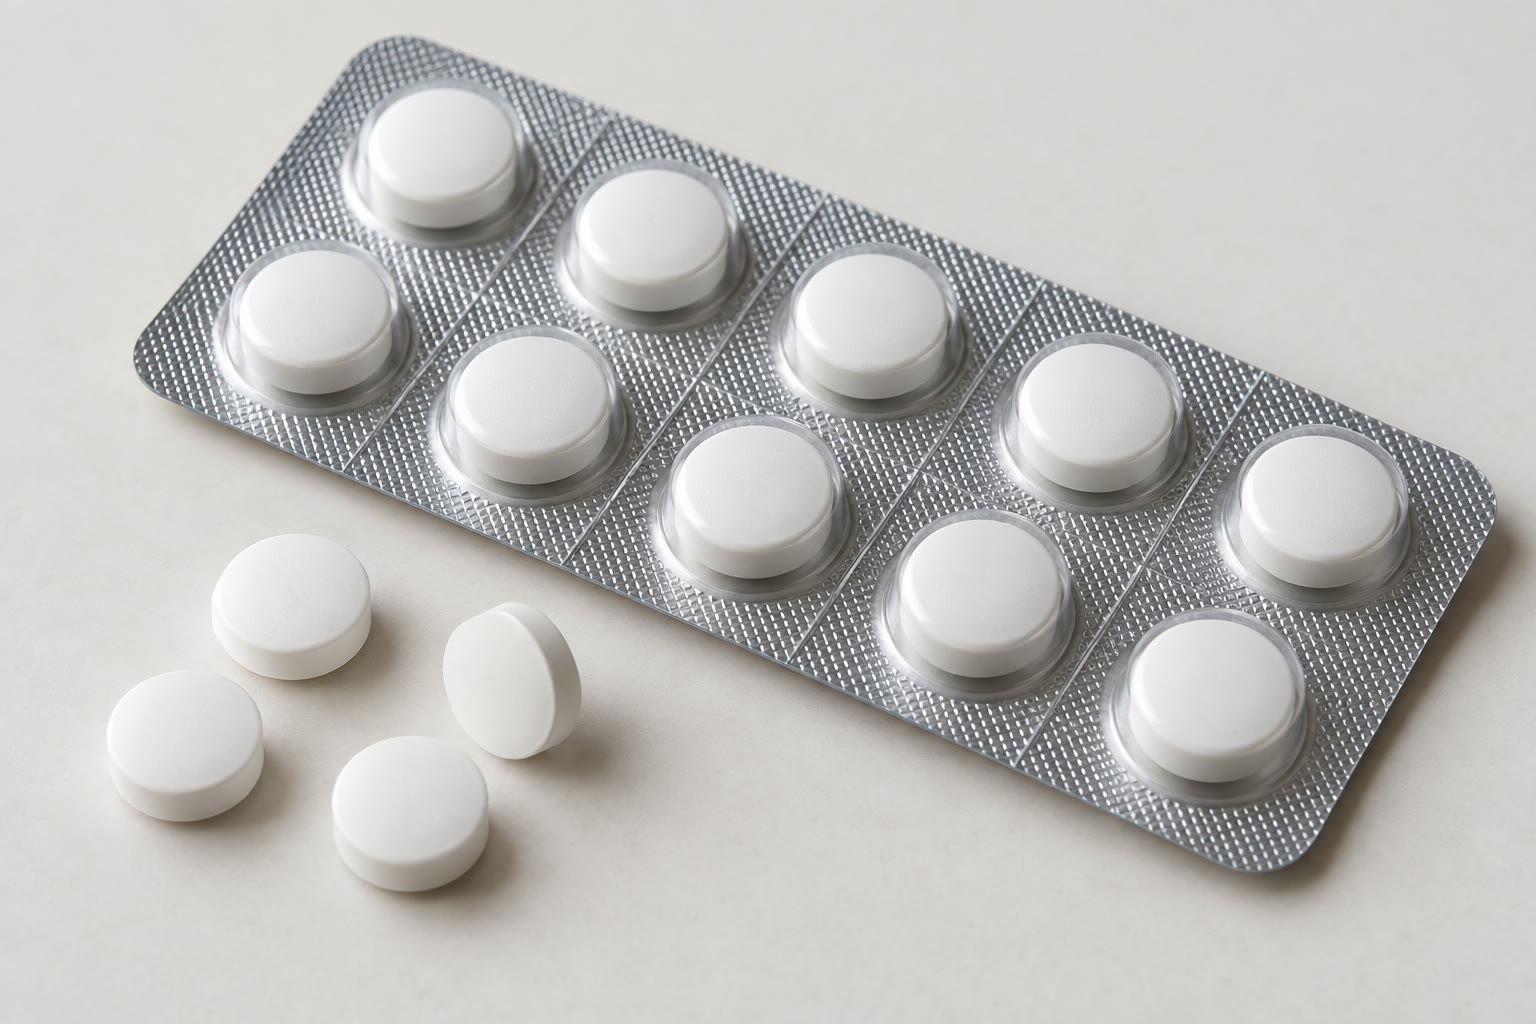
\includegraphics[width=0.45\linewidth]{images/book1/ai/g10-aspirin-tablets.jpg}

{\small Tablet aspirin: masing-masing berisi massa \omterm{def:g6:pure-substances-and-mixtures:pure-substance}{zat murni} yang telah
ditimbang, \omterm{def:g2:mixing-and-dissolving:mix}{dicampur} dengan bahan pengikat.}
\end{omfigure}

\section{Latihan}


\begin{exercise}[$\star$]\label{exo:g10:synthesis-yield:1}
Sebuah \omterm{def:g10:synthesis-yield:synthesis}{sintesis} dapat menghasilkan paling banyak \qty{5.0}{g} produk;
diperoleh \qty{4.2}{g} produk murni dan kering. Hitung \omterm{def:g10:synthesis-yield:yield}{rendemennya}.
\end{exercise}

\begin{exercise}[$\star$]\label{exo:g10:synthesis-yield:2}
Urutkan langkah-langkah \omterm{def:g10:synthesis-yield:synthesis}{sintesis} berikut: mengukur titik leleh;
\omterm{def:g10:synthesis-yield:reflux}{pemanasan dengan refluks}; \omterm{def:g10:synthesis-yield:recrystallisation}{rekristalisasi}; \omterm{def:g10:synthesis-yield:vacuum-filtration}{penyaringan vakum} \omterm{def:g10:synthesis-yield:synthesis}{produk
kasar}; menimbang \omterm{def:g7:chemical-reactions:reactant}{pereaksi}.
\end{exercise}

\begin{exercise}[$\star$]\label{exo:g10:synthesis-yield:3}
Pada rangkaian refluks, mengapa air pendingin dialirkan ke dalam
kondensor dari bawah? Mengapa ujung atas kondensor dibiarkan terbuka?
\end{exercise}

\begin{exercise}[$\star$]\label{exo:g10:synthesis-yield:4}
Dua sifat apa yang harus dimiliki sebuah \omterm{def:g6:solutions-and-solubility:solute}{pelarut} untuk merekristalisasi
sebuah produk? Ke mana pengotornya berakhir?
\end{exercise}

\begin{exercise}[$\star$]\label{exo:g10:synthesis-yield:5}
% ledger: mp:aspirin
Sebuah sampel aspirin hasil \omterm{def:g10:synthesis-yield:synthesis}{sintesis} meleleh antara \qty{124}{\celsius}
dan \qty{130}{\celsius}. Aspirin murni meleleh pada sekitar
\qty{135}{\celsius}. Apakah sampel itu murni? Apa yang harus dilakukan?
\end{exercise}

\begin{exercise}[$\star\star$]\label{exo:g10:synthesis-yield:6}
Sebanyak \qty{2.00}{g} asam salisilat bereaksi dengan anhidrida etanoat
berlebih; diperoleh \qty{2.03}{g} aspirin murni dan kering. Hitung
massa aspirin terbesar dan \omterm{def:g10:synthesis-yield:yield}{rendemennya}.
\end{exercise}

\begin{exercise}[$\star\star$]\label{exo:g10:synthesis-yield:7}
Seorang siswa menimbang aspirinnya selagi masih basah dan memperoleh
\omterm{def:g10:synthesis-yield:yield}{rendemen} \qty{104}{\percent}. Jelaskan. Apakah menimbang \omterm{def:g10:synthesis-yield:synthesis}{produk kasar},
yang tidak dimurnikan tetapi kering, akan memberikan \omterm{def:g10:synthesis-yield:yield}{rendemen} yang
terlalu tinggi atau terlalu rendah dibandingkan \omterm{def:g10:synthesis-yield:yield}{rendemen} sebenarnya?
\end{exercise}

\begin{exercise}[$\star\star$]\label{exo:g10:synthesis-yield:8}
Berikan dua keuntungan \omterm{def:g10:synthesis-yield:vacuum-filtration}{penyaringan vakum} dibandingkan \omterm{def:g3:separating-mixtures:filter}{penyaringan} biasa
melalui kertas saring berbentuk kerucut, untuk mengumpulkan kristal.
\end{exercise}

\begin{exercise}[$\star\star$]\label{exo:g10:synthesis-yield:9}
Pada sebuah pelat kromatografi, garis depan \omterm{def:g6:solutions-and-solubility:solute}{pelarut} telah bergerak
\qty{5.0}{cm}. Bercak produk hasil \omterm{def:g10:synthesis-yield:synthesis}{sintesis} bergerak \qty{3.1}{cm},
bercak aspirin murni \qty{3.1}{cm}, bercak asam salisilat \qty{2.2}{cm}.
Hitung ketiga \omterm{def:g10:chemical-species:retention-factor}{faktor retensinya}. Apa yang dapat disimpulkan tentang
produk itu?
\end{exercise}

\begin{exercise}[$\star\star$]\label{exo:g10:synthesis-yield:10}
\omterm{def:g6:solutions-and-solubility:solubility}{Kelarutan} sebuah produk dalam dua \omterm{def:g6:solutions-and-solubility:solute}{pelarut} adalah:
\begin{center}
\begin{tabular}{lcc}
\hline
\omterm{def:g6:solutions-and-solubility:solute}{pelarut} & dingin (\qty{20}{\celsius}) & panas (mendekati titik didih) \\
\hline
A & \qty{2}{g/L} & \qty{150}{g/L} \\
B & \qty{80}{g/L} & \qty{120}{g/L} \\
\hline
\end{tabular}
\end{center}
\omterm{def:g6:solutions-and-solubility:solute}{Pelarut} mana yang lebih baik untuk \omterm{def:g10:synthesis-yield:recrystallisation}{rekristalisasi}? Untuk \qty{3.0}{g}
\omterm{def:g10:synthesis-yield:synthesis}{produk kasar}, kira-kira berapa volume \omterm{def:g6:solutions-and-solubility:solute}{pelarut} panas yang diperlukan, dan
berapa massa yang paling banyak tetap terlarut setelah dingin?
\end{exercise}

\begin{exercise}[$\star\star$]\label{exo:g10:synthesis-yield:11}
Mengapa labu alas bulat pada rangkaian refluks tidak pernah diisi lebih
dari setengahnya? Mengapa batu didih ditambahkan?
\end{exercise}

\begin{exercise}[$\star\star\star$]\label{exo:g10:synthesis-yield:12}
Sebuah obat dibuat dalam dua langkah, dengan \omterm{def:g10:synthesis-yield:yield}{rendemen}
\qty{80}{\percent} dan \qty{70}{\percent}. Berapa \omterm{def:g10:synthesis-yield:yield}{rendemen}
keseluruhannya? Berapa \omterm{def:g10:synthesis-yield:yield}{rendemen} itu untuk tiga langkah yang
masing-masing \qty{90}{\percent}? Mengapa para ahli kimia berusaha
membuat obat dengan langkah sesedikit mungkin?
\end{exercise}

\begin{exercise}[$\star\star\star$]\label{exo:g10:synthesis-yield:13}
% ledger: sol:aspirin-25
Aspirin \omterm{def:g2:mixing-and-dissolving:dissolve}{larut} dalam air sekitar \qty{3.3}{g/L} pada
\qty{25}{\celsius}. Kristal-kristal dicuci dengan \qty{50}{mL} air pada
suhu itu. Berapa massa aspirin yang paling banyak dapat hilang? Mengapa
air pencucinya didinginkan dalam es terlebih dahulu?
\end{exercise}

\begin{exercise}[$\star\star\star$]\label{exo:g10:synthesis-yield:14}
Sebanyak \qty{2.76}{g} asam salisilat \omterm{def:g2:mixing-and-dissolving:mix}{dicampur} dengan \qty{0.0500}{mol}
anhidrida etanoat. Setelah reaksi, air ditambahkan dan menghancurkan
anhidrida yang berlebih: \ce{C4H6O3 + H2O -> 2C2H4O2}.
\begin{enumerate}
  \item Isilah \omterm{def:g10:reaction-progress-table:extent}{tabel kemajuan} \omterm{def:g10:synthesis-yield:synthesis}{sintesisnya}; berapa jumlah anhidrida yang
        tersisa?
  \item Berapa jumlah total asam etanoat yang ada pada akhirnya?
\end{enumerate}
\end{exercise}

\begin{exercise}[$\star\star\star$]\label{exo:g10:synthesis-yield:15}
Sebuah pabrik harus membuat \qty{1.00}{t} aspirin, dengan \omterm{def:g10:synthesis-yield:yield}{rendemen}
keseluruhan \qty{85}{\percent} dari asam salisilat. Berapa massa asam
salisilat yang harus dibelinya?
\end{exercise}

\section{Soal: Membuat Aspirin}

\begin{problem}[{Soal akhir pekan --- dari tiga gram asam salisilat sampai
sestoples aspirin murni: berapa rendemennya?}]
\label{pb:g10:synthesis-yield:1}
% ledger: rho:acetic-anhydride, mp:aspirin, mp:salicylic, sol:aspirin-25, aw:C, aw:H, aw:O
Sebuah kelas membuat aspirin. Di dalam labu: \qty{3.0}{g} asam
salisilat dan \qty{6.0}{mL} anhidrida etanoat, dengan massa jenis
\qty{1.08}{g/mL}, ditambah beberapa tetes asam; \omterm{def:g6:pure-substances-and-mixtures:mixture}{campuran} itu dipanaskan
dengan refluks. \omterm{def:g10:synthesis-yield:synthesis}{Produk kasar} yang dikumpulkan dengan \omterm{def:g10:synthesis-yield:vacuum-filtration}{penyaringan vakum}
beratnya \qty{3.6}{g} dalam keadaan basah dan \qty{3.3}{g} setelah
kering. Setelah \omterm{def:g10:synthesis-yield:recrystallisation}{rekristalisasi} dan pengeringan, tersisa \qty{2.7}{g}
kristal putih.

\medskip
\noindent\textbf{Bagian I --- Reaksinya.}
\begin{enumerate}
  \item Periksalah bahwa persamaan
        \ce{C7H6O3 + C4H6O3 -> C9H8O4 + C2H4O2} setara.
  \item Hitung \omterm{def:g10:the-mole:molar-mass}{massa molar} asam salisilat, anhidrida etanoat, aspirin,
        dan asam etanoat.
  \item Sebutkan \omterm{def:g7:chemical-reactions:reactant}{pereaksi-pereaksinya}, produk yang diinginkan, dan produk
        sampingnya.
  \item Mengapa \omterm{def:g6:pure-substances-and-mixtures:mixture}{campuran} itu dipanaskan dengan refluks dan bukan di dalam
        labu terbuka?
\end{enumerate}

\medskip
\noindent\textbf{Bagian II --- Massa terbesar.}
\begin{enumerate}[resume]
  \item Hitung jumlah awal asam salisilat.
  \item Hitung massa, lalu \omterm{def:g10:the-mole:amount}{jumlah zat}, anhidrida etanoat.
  \item Isilah \omterm{def:g10:reaction-progress-table:extent}{tabel kemajuannya}. \omterm{def:g7:chemical-reactions:reactant}{Pereaksi} mana yang membatasi? Berikan
        $x_{\max}$.
  \item Simpulkan massa aspirin terbesar.
  \item Mengapa anhidridanya, dan bukan asam salisilatnya, yang dibuat
        berlebih?
\end{enumerate}

\medskip
\noindent\textbf{Bagian III --- Mengisolasi dan memurnikan.}
\begin{enumerate}[resume]
  \item Mengapa massa basah, \qty{3.6}{g}, tidak dapat dipakai untuk
        menghitung \omterm{def:g10:synthesis-yield:yield}{rendemen}?
  \item Hitung \omterm{def:g10:synthesis-yield:yield}{rendemen} \omterm{def:g10:synthesis-yield:synthesis}{produk kasar} yang kering.
  \item Mengapa \omterm{def:g10:synthesis-yield:recrystallisation}{rekristalisasi} menurunkan massanya?
  \item Kristal-kristal itu dicuci dengan \qty{30}{mL} air pada
        \qty{25}{\celsius}, suhu ketika aspirin \omterm{def:g2:mixing-and-dissolving:dissolve}{larut} sekitar
        \qty{3.3}{g/L}. Berapa massa yang paling banyak dapat hilang
        dengan cara ini?
  \item Hitung \omterm{def:g10:synthesis-yield:yield}{rendemen} produk murninya.
\end{enumerate}

\medskip
\noindent\textbf{Bagian IV --- Memeriksa produknya.}
\begin{enumerate}[resume]
  \item Kristal hasil \omterm{def:g10:synthesis-yield:recrystallisation}{rekristalisasi} meleleh dengan tajam pada
        \qty{135}{\celsius}. Apa yang ditunjukkan hal ini?
  \item \omterm{def:g10:synthesis-yield:synthesis}{Produk kasarnya} meleleh antara \qty{120}{\celsius} dan
        \qty{131}{\celsius}. Apa yang ditunjukkan hal ini?
  \item Pada pelat kromatografi, \omterm{def:g10:synthesis-yield:synthesis}{produk kasar} memberikan dua bercak,
        satu setinggi aspirin murni dan satu setinggi asam salisilat;
        produk hasil \omterm{def:g10:synthesis-yield:recrystallisation}{rekristalisasi} memberikan satu bercak, setinggi
        aspirin. Simpulkan.
  \item Bercak produk hasil \omterm{def:g10:synthesis-yield:recrystallisation}{rekristalisasi} bergerak \qty{3.1}{cm} dan
        garis depan \omterm{def:g6:solutions-and-solubility:solute}{pelarut} \qty{5.0}{cm}. Hitung \omterm{def:g10:chemical-species:retention-factor}{faktor retensinya}.
  \item Antara reaksi dan \omterm{def:g10:synthesis-yield:recrystallisation}{rekristalisasi}, bagian pekerjaan mana yang
        lebih banyak kehilangan aspirin?
  \item Nyatakan jawaban akhirnya: berapa \omterm{def:g10:synthesis-yield:yield}{rendemen} \omterm{def:g10:synthesis-yield:synthesis}{sintesis} ini?
\end{enumerate}
\end{problem}
